\section{Quantum Algorithnms}

\todo{add start of lecture 14/12}


Quantum version of $f$?
$\leadsto$ Quantum "oracle" $U_f$ defined for computational basis states as

\begin{figure}[H]
    \centering
    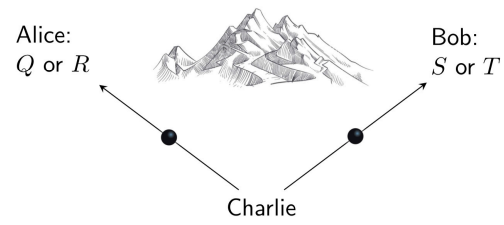
\includegraphics[scale=0.5]{chapters/res/alice-bob-charlie-mountain.png}
    \caption{\todo{Add quantum circuit representation of $U_f$}}
\end{figure}

Note: $U_f$ maps basis states to basis states and satisfies 
\begin{equation}
U_f^2 = I \quad (\text{since } q \oplus f(x) \oplus f(x) = q)
\end{equation}

Thus $U_f$ permutes basis states and is in particular unitary. \\
\newline

Initialize oracle qubit in superposition $\ket{-} = \frac{1}{\sqrt{2}}(\ket{0} - \ket{1})$, 
then 

\begin{equation}
    \ket{x} \otimes \frac{\ket{0} - \ket{1}}{\sqrt{2}}
    \stackrel{U_f}{\mapsto}
    \begin{cases}
        \ket{x} \otimes \frac{\ket{0} - \ket{1}}{\sqrt{2}} & \text{if } f(x) = 0\\
        \ket{x} \otimes \frac{\ket{1} - \ket{0}}{\sqrt{2}} = 
            - \ket{x} \otimes \frac{\ket{0} - \ket{1}}{\sqrt{2}} & \text{if } f(x) = 1
    \end{cases}
\end{equation}

In summary: 
\begin{equation}
    \ket{x} \otimes \frac{\ket{0} - \ket{1}}{\sqrt{2}}
    \stackrel{U_f}{\mapsto}
    \underbrace{{\color{blue}-1^{f(x)}}}_{\text{only this part relevant for the following}}
        \ket{x} \otimes \underbrace{\frac{\ket{0} - \ket{1}}{\sqrt{2}}}_{\text{Oracle qubit unchanged}}
\end{equation}

$\leadsto$ Effective action of oracle

\begin{figure}[H]
    \centering
    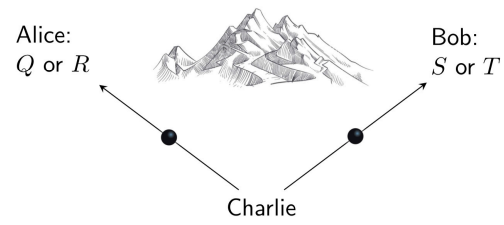
\includegraphics[scale=0.5]{chapters/res/alice-bob-charlie-mountain.png}
    \caption{\todo{Add Quantum oracle solution diagram}}
\end{figure}


How could one construct such an oracle without knowing solution already? \\
Example: Factorization of a large integer $m \in \mathbb{N}$:
Finding prime factor of $m$ is "difficult" on a classical computer (no known algorithm with
polynomial runtime in the bit length of $m$). \\
But testing whether a given $x \in \mathbb{N}$ divides $m$ is simple.

Can perform arithmeti operations for trial divisions on a digital quantum computer as well
$\leadsto$ Oracle which recognizes a solution $x$.

\subsection{Grover's Algorithm}
Search space with $N = 2^n$ elements, $M$ solutions. 

\begin{figure}[H]
    \centering
    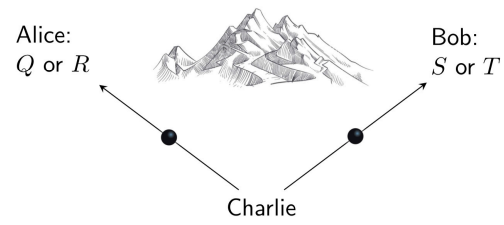
\includegraphics[scale=0.5]{chapters/res/alice-bob-charlie-mountain.png}
    \caption{\todo{Add Grovers algorithm quantum circuit}}
\end{figure}

Initial Hadamard transform: \\

\begin{figure}[H]
    \centering
    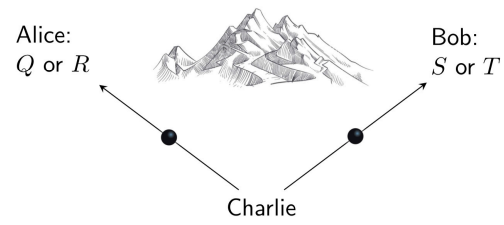
\includegraphics[scale=0.5]{chapters/res/alice-bob-charlie-mountain.png}
    \caption{\todo{Add initial hadamard circuit}}
\end{figure}

Applied to several qubits:

\begin{align}
    H^{\otimes n} \ket{x_1, ..., x_n} 
        &= \underbrace{(H\ket{x_1})}_{\frac{1}{\sqrt{2}} \sum_{z_1 = 0}^1 (-1)^{x_1 z_1} \ket{z_1}}
            \otimes \cdots \otimes (H \ket{x_n}) \\ 
        % 
        &= \frac{1}{\sqrt{2^n}}  \sum_{z = 0}^{2^n - 1} (-1)^{x \cdot z} \underbrace{\ket{z}}_{\text{bit string}}
\end{align}

In particular: 
\begin{equation}
    H^{\otimes n} \ket{0, ..., 0} = \frac{1}{\sqrt{N}} \sum_{z = 0}^{N} \ket{z} =: \color{green} \statepsi
\end{equation}

Definition of Grover operator G:

\begin{figure}[H]
    \centering
    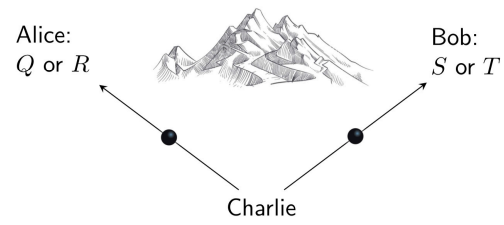
\includegraphics[scale=0.5]{chapters/res/alice-bob-charlie-mountain.png}
    \caption{\todo{Add Grover operator circuit}}
\end{figure}

In summary 
\begin{equation}
    G := (2 \statepsi \bra{\psi} - I) U_f
\end{equation}


\underline{Geometric interpretation}

\begin{figure}[H]
    \centering
    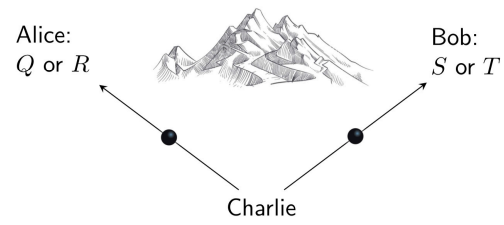
\includegraphics[scale=0.5]{chapters/res/alice-bob-charlie-mountain.png}
    \caption{\todo{Add grover geometric representation}}
\end{figure}


Define 
\begin{equation}
    \ket{\alpha} := \frac{1}{\sqrt{N - M}} \sum_{x=0, f(x) = 0}^N \ket{x}
\end{equation}

\begin{equation}
    \ket{\beta} := \frac{1}{\sqrt{M}} \sum_{x=0, f(x) = 1}^N \ket{x}
\end{equation}


Angle $\vartheta$ defined by $\sin \frac{\vartheta}{2} = \sqrt{\frac{N}{M}}$
such that $\statepsi = \cos \frac{\vartheta}{2} \ket{\alpha} + \sin \frac{\vartheta}{2} \ket{\beta}$

Note: By definition $U_f \ket{a} = \alpha$, $U_f \ket{\beta} = -\ket{\beta}$ \\
$\leadsto U_f$ is a reflection about $\ket{\alpha}$ within subspace spanned by $\ket{\alpha}$ and $\ket{\beta}$ \\

Likewise $2 \statepsi \bra{\psi} - I$ is a reflection about $\statepsi$

\begin{figure}[H]
    \centering
    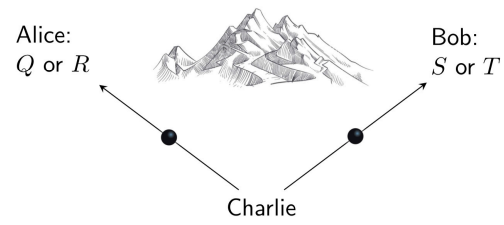
\includegraphics[scale=0.5]{chapters/res/alice-bob-charlie-mountain.png}
    \caption{\todo{Add $\psi$ reflection diagram}}
\end{figure}

Since $\statepsi$ is part of subspace spanned by $\ket{\alpha}$ and $\ket{\beta}$, 
$G$ leaves subspace invariant! \\
Thus $G$ is a product of two reflections $\leadsto G$ is a rotation by angle 
$\vartheta$
\begin{align}
    \ket{\phi} &= \cos{\varphi} \ket{\alpha} + \cos{\varphi} \ket{\beta} \\
    \leadsto G \ket{\phi} &= \cos{(\varphi + \vartheta)} \ket{\alpha} + \cos{(\varphi + \vartheta)} \ket{\beta}
\end{align}